	\documentclass[12pt,a4paper,italian]{article}


\usepackage[italian]{babel}
\usepackage[latin1]{inputenc}
\usepackage{amsmath}
\usepackage{amsfonts}
\usepackage{amssymb}
\usepackage{color}
\usepackage{xcolor}
\usepackage{hyperref}
\usepackage[all]{hypcap}
\usepackage{ifthen}
\usepackage{wrapfig}
%\author{Piero Bizzotto}
\usepackage[top=2cm,bottom=5cm,left=80pt,right=80pt]{geometry}
\usepackage{graphicx}
\DeclareGraphicsExtensions{.jpg,.png}

\newcommand{\ajax}{AJAXDRAW}
\newcommand{\sito}{\href{http://ajaxdraw.sourceforge.net}{http://ajaxdraw.sourceforge.net}}

\setlength{\parindent}{0pt} %settato indentazione di default 
\setlength{\headheight}{3cm} %settato grandezza header...in altre parole, quanto distanzio il doc dall'intestazione

\usepackage{fancyhdr} %pacchetto per le intestazioni
\pagestyle{fancy} %uso del pacchetto


\fancyhead{} %annulla head di default
\fancyfoot{} %annulla foot di default


\usepackage{lastpage} %setto pg di pgtot a rfoot
     \rfoot{pagina \thepage\ di \pageref{LastPage}}


\lfoot{Versione: \insertversion} %setto versione doc a lfoot
\renewcommand{\footrulewidth}{0.5pt} %ridefinisco il valore della riga di intestazione
\renewcommand{\headrulewidth}{0.5pt} %ridefinisco il valore della riga di pie' di pagina

\newcommand{\insertversion}{0.0} %definisco il nuovo comando per inserire la versione


\lhead{  \begin{Huge} \ajax \end{Huge} \\  %intestazione di sinistra
					%\begin{Large}	Software per il Disegno Grafico\\ in Tecnologie Web \end{Large}  
					\begin{normalsize}\sito \end{normalsize}
			%\\ versione documento: \insertversion\ del \today} %setto l'intestazione sx
		}
\rhead{ %includo logo nell'intestazione dx
	 	
\includegraphics[scale=0.5]{../logo/logo.png}  
}


%CREAZIONE ELENCHI NUMERATI PERSONALIZZATI
\newcounter{Lcount}
\newcounter{Rcount}
\setcounter{Lcount}{0}
\setcounter{Rcount}{0}

\newenvironment{elenconumerato}[2][ ]
{
  \begin{list}{#1\arabic{Lcount}.}
    {
	\setcounter{Rcount}{\value{Lcount}}
	\setcounter{Lcount}{0} 
	\usecounter{Lcount} 
\addtolength{\leftmargin}{#2pt}
	}
}
{
  \end{list}
 \setcounter{Lcount}{\value{Rcount}}
}

%CREAZIONE ELENCHI PUNTATI
\newenvironment{elencopuntato}[1][]
{
\begin{list}{\textbullet} %\itemindent=#1pt
	{
	\addtolength{\leftmargin}{#1pt}
	}
} 
{
\end{list}
}


\newenvironment{elencodescrittivo}[1][]{\begin{description} \setlength{\itemindent}{#1pt} \addtolength{\leftmargin}{#1pt}} {\end{description}}

\newcommand{\TITOLODOC}{Titolo}

%footer centrale
\cfoot{ \TITOLODOC \\  E-mail:    \href{ mailto:webshape.contact@gmail.com}{ webshape.contact@gmail.com}  }

%INSERIMENTO IMMAGINI
\newcommand{\imagerealsize}[1]{\vspace{20pt} \includegraphics{#1} }
\newcommand{\imageadapted}[1]{\vspace{20pt} \includegraphics[width=1\textwidth]{#1} }

\newcommand{\glosspath}{.\glossario}
\newcommand{\gloss}[1]{\hyperref{\glosspath~\glossario.pdf}{}{#1}{#1}}

\hypersetup{
    %bookmarks=true,         % show bookmarks bar?
    %unicode=false,          % non-Latin characters in Acrobat’s bookmarks
	%pdftoolbar=true,        % show Acrobat’s toolbar?
	%pdfmenubar=true,        % show Acrobat’s menu?
    %pdffitwindow=true,      % page fit to window when opened
    %pdftitle={My title},    % title
    %pdfauthor={Author},     % author
    %pdfsubject={Subject},   % subject of the document
    %pdfnewwindow=true,      % links in new window
    %pdfkeywords={keywords}, % list of keywords
    colorlinks=true,         % false: boxed links; true: colored links
    linkcolor=black,           % color of internal links
    %citecolor=green,        % color of links to bibliography
    %filecolor=magenta,      % color of file links
    urlcolor=teal    % color of external links
%	linktocpage=false;
}


%COLORAZIONE TESTO
\newcommand{\blue}[1]{{\color {blue} #1}} 
\newcommand{\red}[1]{{\color {red} #1}}
\newcommand{\green}[1]{{\color {green} #1}}
\newcommand{\sezione}[1]{\leftskip=0pt \section{#1} \leftskip=18pt}
\newcommand{\subsezione}[1]{\leftskip=18pt \subsection{#1} \leftskip=36pt}
\newcommand{\subsubsezione}[1]{\leftskip=36pt \subsubsection{#1} \leftskip=54pt}
\newcommand{\subsubsecindent}{54}
\newcommand{\subsecindent}{36}
\newcommand{\secindent}{18}
\newcommand{\normindent}{8}
\newcommand{\code}[1]{{\bfseries \texttt{#1}}}
\newcommand{\paragrafo}[1]{\leftskip=36pt \paragraph{#1} \leftskip=54pt}
\newcommand{\subparagrafo}[1]{\leftskip=54pt \subparagraph{#1} \leftskip=72pt} %BASE!!!
\usepackage{multirow}
\title{\TITOLODOC}
\author{Dal Bosco Davide}

\begin{document}

\renewcommand{\insertversion}{3.1} %INSERIRE LA VERSIONE QUI DENTRO STILE x.x.xx
\renewcommand{\TITOLODOC}{Piano di Progetto} %INSERIRE IL TITOLO DEL DOCUMENTO DA FAR COMPARIRE A PIE PAGINA
\renewcommand{\glosspath}{.\glossario} %INSERIRE PERCORSO RELATIVO

%%%%%%%%%%%%%%%%%%%%%%PARTE DA NON MODIFICARE%%%%%%%%%%%%%%%%%
\begin{titlepage}
\begin{center}
	\begin{Large}	\today \end{Large}
\end{center}

\vspace{20pt}

\begin{center}
	\begin{Huge}
				\textbf{\ajax}
	\end{Huge}
\end{center}			

\begin{center}
	\begin{large}
				\textbf{Software per il Disegno Grafico\\ in Tecnologie Web}
	\end{large}
\end{center}			

\vspace{20pt}

\begin{center}

\includegraphics[width=150pt]{../logo/logo}
\end{center}

\vspace{170pt}
\begin{center} %INSERIRE ALL'INTERNO IL TITOLO DOCUMENTO CHE COMPARIRA NELLA PAGINA INIZIALE				
	\begin{Huge}
				\textbf{\TITOLODOC}
	\end{Huge}
			\\
\end{center}
\vspace{190pt}
\begin{center}
Versione: \insertversion
\end{center}
\end{titlepage}

\newpage
%%%%%%%%%%%%%%%%%%%%%%FINE PARTE DA NON MODIFICARE%%%%%%%%%%%%%%%%%

\begin{center} %INSERIRE ALL'INTERNO IL TITOLO DOCUMENTO CHE COMPARIRA NELLA PAGINA INIZIALE
	\begin{Huge}	
				\textbf{\TITOLODOC}
			\\
	\end{Huge}
\end{center}

%\setlength{\parindent}{18pt} %settato indentazione di default 
\section*{\LARGE Sommario:}
Il presente documento descrive l'analisi dei costi e delle risorse effettuata dall'azienda WebShape per lo sviluppo del Capitolato C04.

 %SEZIONE SOMMARIO
\indent \indent

\section*{\LARGE Stato del documento:}
\indent \indent
	Formale Esterno

\section*{\LARGE Redazione:}
	\begin{table}[!h]
		\begin{center}
			\begin{tabular}
				{|c|c|}
				\hline
				%%%%%%%%%%%%%%INTESTAZIONE COLONNE%%%%%%%%%%%%%%%%%%%%%%%%%%%%%%%%
				\multicolumn{2}{|c|}{ \textbf{Redazione} } \\
				\hline
				\textbf{Fase} & \textbf{Redattori} \\
				%%%%%%%%%%%%%%FINE INTESTAZIONE COLONNE%%%%%%%%%%%%%%%%%%%%%%%%%%%%%%%%%%%%%%
				\hline
				%%%%%%%%%%% PARTE DA MODIFICARE %%%%%%%%%%%%%%%%%%%%%%%%%%%%%%%%%%%%%%%%%%		
				\multirow{2}{*}{Pre-RR} & Cunico Marco\\
										& Dal Bosco Davide\\
				\hline
				RR-RPP & Bizzotto Piero\\
				\hline
				RPP-RQ & Geremia Mirco\\
				\hline
				%%%%%%%%%%% FINE PARTE DA MODIFICARE %%%%%%%%%%%%%%%%%%%%%%%%%%%
			\end{tabular}
			\caption{Lista Redattori} %INSERIRE DIDASCALIA - SE NECESSARIA - 
			\label{tabredazione}
		\end{center}
	\end{table}
	
	
\section*{\LARGE Verifica:}
\begin{table}[!h]
	\begin{center}
		\begin{tabular}
			{|c|c|}
			\hline
			%%%%%INTESTAZIONE COLONNE%%%%%%%%%%%%%%%%%%%%%%%%%%%%%%%
			\multicolumn{2}{|c|}{ \textbf{Verifica} } \\
			\hline
			\textbf{Fase} & \textbf{Verificatori} \\
			%%%%%%%%%%%%%%FINE INTESTAZIONE COLONNE%%%%%%%%%%%%%%%%%%%%%%%%%%%%%%
			\hline
			%%%%%%%%%%% PARTE DA MODIFICARE %%%%%%%%%%%%%%%%%%%%%%%%%%%%%%%%%%%%%%		
			Pre-RR & Geremia Mirco \\
			\hline
			RR-RPP & Geremia Mirco\\
			\hline
			RPP-RQ & Carollo Mirko \\									
			\hline
			%%%%%%%%%%% FINE PARTE DA MODIFICARE %%%%%%%%%%%%%%%%%%%%%%%%%%%%%%%%%%%
		\end{tabular}
		\caption{Lista Verificatori} %INSERIRE DIDASCALIA - SE NECESSARIA - 
		\label{tabverifica}
	\end{center}
\end{table}	
	
\section*{\LARGE Approvazione:}
\begin{table}[!h]
	\begin{center}
		\begin{tabular}
			{|c|c|}
			\hline
			%%%%%INTESTAZIONE COLONNE%%%%%%%%%%%%%%%%%%%%%%%%%%%%%%%
			\multicolumn{2}{|c|}{ \textbf{Approvazione} } \\
			\hline
			\textbf{Fase} & \textbf{Approvatori} \\
			%%%%%%%%%%%%%%FINE INTESTAZIONE COLONNE%%%%%%%%%%%%%%%%%%%%%%%%%%%%%%
			\hline
			%%%%%%%%%%% PARTE DA MODIFICARE %%%%%%%%%%%%%%%%%%%%%%%%%%%%%%%%%%%%%%		
			Pre-RR & Dissegna Stefano \\
			\hline
			RR-RPP & Bizzotto Piero\\
			\hline
			RPP-RQ & Rizzo Maurizio \\
			\hline
			%%%%%%%%%%% FINE PARTE DA MODIFICARE %%%%%%%%%%%%%%%%%%%%%%%%%%%%%%%%%%%
		\end{tabular}
		\caption{Lista Approvatori} %INSERIRE DIDASCALIA - SE NECESSARIA - 
		\label{tabapprovazione}
	\end{center}
\end{table}

\textbf{}
\section*{\LARGE Lista di Distribuzione:}

	\begin{elenconumerato}{\normindent}
		\item WebShape 
		\item I committenti Conte Renato e Vardanega Tullio in rappresentanza \\  dell'azienda proponente Zucchetti SPA
	\end{elenconumerato}

\newpage


\section*{\Large Registro delle Modifiche:}


\begin{center}
	\begin{table}[h]
		  \begin{tabular*}
			{1\textwidth}%
				{@{\extracolsep{\fill}}|p{0.1\textwidth}|p{0.54\textwidth}|p{0.26\textwidth}|}
			 \hline
%%%%%%%%%%%%%%INTESTAZIONE COLONNE%%%%%%%%%%%%%%%%%%%%%%%%%%%%%%%%%%%%%%%%%%
			\textbf{Versione}  & \textbf{Descrizione} & \textbf{Autore} \\
%%%%%%%%%%%%%%FINE INTESTAZIONE COLONNE%%%%%%%%%%%%%%%%%%%%%%%%%%%%%%%%%%%%%%%
		 \hline
%%%%%%%%%%% PARTE DA MODIFICARE %%%%%%%%%%%%%%%%%%%%%%%%%%%%%%%%%%%%%%%%%%%
			3.1 & 19/03/2009 Modifiche al consuntivo fase RPP-RQ & \\
			\hline
			3.0 & 07/03/2009 Verifica in preparazione al rilascio & Geremia Mirco\\
			\hline
			2.2 & 04/03/2009 Aggiunto consuntivo fase RPP-RQ & Geremia Mirco\\
            \hline
            2.1 & 13$\slash$02$\slash$2009    Modifiche post integrazione  & Rizzo Maurizio \\
            \hline
			2.0 & 23/01/2009	Verifica in preparazione al rilascio & Bizzotto Piero \\
			\hline
			1.2 & 21/01/2009	Aggiunta consuntivi fase RR-RPP & Bizzotto Piero \\
			\hline
			1.1 & 17/01/2009	Aggiornamento in seguito all'esito della Revisione dei Requisiti & Bizzotto Piero \\
			\hline
			1.0 & 	 09$\slash$12$\slash$2008 Verifica finale in preparazione al rilascio & Cunico Marco \\
			\hline
          0.9 & 06/12/2008 Inserito secondo incremento e fine stesura del documento & Dal Bosco Davide\\
          \hline
          0.8 & 06/12/2008 Corretti errori di sintassi, impaginazione e inserito il primo incremento & Cunico Marco \\
		 \hline
          0.7 & 05/12/2008 Inserimento Distribuzione Ruoli e Gestione del Piano di Progetto & Cunico Marco \\
          \hline
          0.6 & 05/12/2008 Inserimento Preventivo Rotazione Ruoli per fase di progetto & Cunico Marco \\
          \hline
          0.5 & 05/12/2008 Inserimento della sezione relativa all'Analisi e Gestione dei Rischi & Dal Bosco Davide \\
          \hline         
          0.4 & 04/12/2008 Inserimento attribuzione ruoli & Cunico Marco \\
          \hline	          
          0.3 & 04/12/2008 Inserimento intero capitolo Pianificazione con relative sottosezioni, tabelle e grafici & Dal Bosco Davide \\
          \hline
    	  0.2 & 01/12/2008 Inserimento capitoli Introduzione, Organigramma, Pianificazione(inizio) & Dal Bosco Davide \\
    	  \hline
    	  0.1 & 25/11/2008 Adattamento al template scelto & Dal Bosco Davide \\
    	  \hline
    	  0.0 & 22/11/2008 Bozza iniziale & Dal Bosco Davide \\

		\hline %%FINE RIGA
%%%%%%%%%%% FINE PARTE DA MODIFICARE %%%%%%%%%%%%%%%%%%%%%%%%%%%%%%%%%%%%%
		\end{tabular*}
	\caption{Registro delle modifiche} %INSERIRE DIDASCALIA - SE NECESSARIA - 
	\label{tab:modifiche}
	\end{table}
\end{center}


\newpage
\thispagestyle{fancy}
\tableofcontents
\thispagestyle{fancy}
\newpage

\sezione{Introduzione}

\subsezione{Scopo del documento}
Il documento si propone di presentare ai Committenti le scelte effettuate riguardanti la distribuzione dei ruoli e delle risorse, l'assegnazione delle attivit\`a dei componenti dell'azienda e lo studio dei costi necessari per la realizzazione del progetto inerente al capitolato d'appalto C04.\\

\sezione{Organigramma}
In data 15 ottobre 2008 \`e stato costituito il gruppo WebShape formato da sei membri, tutti in possesso delle idoneit\`a necessarie per partecipare al progetto di Ingegneria del Software.
I ruoli saranno assegnati a rotazione nell'arco dello sviluppo del progetto, in base alle disponibilit\`a dei componenti del gruppo.\\

\subsezione{Accettazione}
\begin{table}[h]
	\begin{center}
		  \begin{tabular}{|p{0.3\textwidth}|l|p{0.3\textwidth}|}
		 \hline 
		 \textbf{Cognome e Nome} & \textbf{Data} & \textbf{Firma}\\
		 \hline
		Bizzotto Piero & 15-10-2008 & \\
		\hline
		Carollo Mirko & 15-10-2008 & \\
		\hline
		Cunico Marco & 15-10-2008 & \\
		\hline
		Dal Bosco Davide & 15-10-2008 & \\
		\hline
		Dissegna Stefano & 15-10-2008 & \\
		\hline
		Geremia Mirco & 15-10-2008 & \\
		\hline
		Rizzo Maurizio & 7-1-2009 & \\
		\hline
		\end{tabular}
	\caption{Accettazione} 
	\label{tabella_accettazione}
	\end{center}	
\end{table}

\newpage

\subsezione{Descrizione Componenti}
%(\ref{tab:tabella_componenti}) della pagina ~\pageref{tab:tabella_componenti}\\

\begin{table}[h]
	\begin{center}
		  \begin{tabular}{|p{0.3\textwidth}|l|l|}
		 \hline 
		 \textbf{Cognome e Nome} & \textbf{Matricola} & \textbf{E-mail}\\
		 \hline
		Bizzotto Piero & 540804 & piero.bizzotto@gmail.com \\
		\hline
		Carollo Mirko & 542902 & mirko.carollo@gmail.com\\
		\hline
		Cunico Marco & 540754 & marco.cunico@gmail.com\\
		\hline
		Dal Bosco Davide & 539402 & mrdavi86@gmail.com\\
		\hline
		Dissegna Stefano & 561011 & stefano.dissegna@gmail.com \\
		\hline
		Geremia Mirco & 563665 & crittico@gmail.com\\
		\hline
		Rizzo Maurizio & 479720 & clue.manari@gmail.com\\
		\hline
		\end{tabular}
	\caption{Descrizione dei Componenti} 
	\label{tab:tabella_componenti}
	\end{center}	
\end{table}


\subsezione{Assunzioni Iniziali}
\begin{itemize}
\item Il costo totale stimato \`e di 13770 euro. Eventuali costi aggiuntivi non saranno a carico del committente ma saranno coperti dall'azienda.
\item Sono previste 669 ore di lavoro totali per la realizzazione del progetto.
\item L'impegno individuale di ogni componente varia da un minimo di 90 ore ad un massimo di 100 ore.
\end{itemize}


\subsezione{Attribuzione dei Ruoli}
Date le Assunzioni Iniziali precedentemente descritte, ed essendo il gruppo WebShape costituito da sette membri, si avr\`a una media di circa 95 ore di lavoro per persona. La durata complessiva del progetto sar\`a di circa 669 ore, ogni componente lavorer\`a quindi una media di circa 2 ore giornaliere. Sono previste altre tre revisioni:
\begin{elenconumerato}{\normindent}
				\item Revisione di Progetto Preliminare (RPP)
				\item Revisione di Qualifica (RQ)
				\item Revisione di Accettazione (RA)
			\end{elenconumerato}

La rotazione dei ruoli avviene come da tabelle (\ref{tab:TabellaRotazRuoliUno}) e (\ref{tab:TabellaRotazRuoliDue}) a pagina ~\pageref{tab:TabellaRotazRuoliUno}.\\
Dato che ogni componente del gruppo dovr\`a assumere tutti i ruoli, \`e previsto che nelle varie fasi del progetto i membri della societ\`a si assumano pi\`u incarichi. Non \`e permesso che uno stesso membro ricopra ruoli in conflitto di interessi tra loro.\\

\sezione{Pianificazione}
Per la realizzazione del progetto l'azienda WebShape ha valutato con attenzione i possibili modelli di cicli di vita da utilizzare, tenendo conto di eventuali pregi e difetti. 
La scelta \`e ricaduta sul modello incrementale, in quanto, vista la tipologia modulare del progetto, si adatta meglio alle esigenze dell'azienda stessa. Con il modello incrementale si ha la possibilit\`a di effettuare dei rilasci di versioni parziali in modo da avvicinarsi incrementalmente al prodotto finale ed effettuare una pianificazione ben definita, che sono dei vantaggi importanti per una nuova azienda. Sono stati invece scartati gli altri modelli: il modello sequenziale, perch\`e troppo orientato ai documenti e per il fatto che il primo prodotto del progetto \`e visionabile solo al termine della Fase di Qualifica; il modello evolutivo, per la necessit\`a di un costante rilascio di versioni; infine il modello a spirale, per l'esigenza di avere continui contatti col cliente.\\
\subsezione{Ore e costi totali}
In questa sottosezione verr\`a illustrato il preventivo totale, comprendente i costi e le ore stimate necessarie per la realizzazione del progetto. Il preventivo considera tutte le fasi di progettazione sostenute dall'azienda.

\begin{table}[h]
	\begin{center}
		  \begin{tabular}{|c|c|c|c|}
		 \hline 
		 \textbf{Ruolo} & \textbf{Ore di lavoro} & \textbf{Costo in euro}\\
		 \hline
		Responsabile & 66 & 1980 \\
		Amministratore & 87 & 1740\\
		Analista & 98 & 2450\\
		Progettista & 152 & 3344\\
		Programmatore & 107 & 1712 \\
		Verificatore & 159 & 2544\\
        \hline
        \textbf{Totale} & \textbf{669} & \textbf{13770}\\
		\hline
		\end{tabular}
	\caption{Preventivo totale} 
	\label{tab:tabella_preventivo}
	\end{center}	
\end{table}

\newpage
\begin{center}\textbf{Ore/Ruolo}
\end{center}
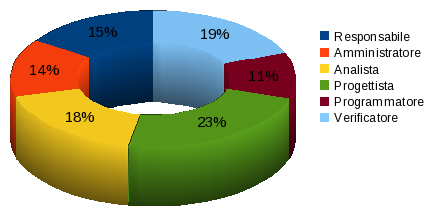
\includegraphics[width=300pt]{Ore_Totali}

\begin{center}\textbf{Costo/Ruolo}
\end{center}
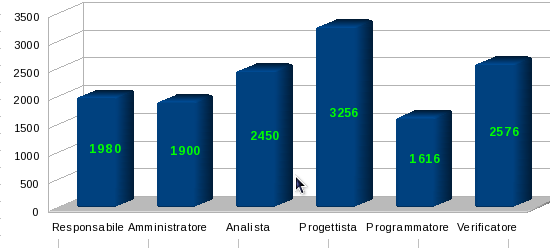
\includegraphics[width=300pt]{Costi_Totali}

\newpage

\subsezione{Pianificazione economico-temporale RR-RPP}
All'interno di questa fase si concluder\`a la fase di analisi e inizier\`a quella di progettazione, con la definizione di un progetto di massima che si svilupper\`a e concretizzer\`a nelle due iterazioni previste all'interno della fase RPP-RQ, descritta in seguito. \\
\\
Preventivo relativo alla fase Revisione dei requisiti-Revisione del progetto preliminare.
\begin{table}[h]
	\begin{center}
		  \begin{tabular}{|c|c|c|c|}
		 \hline 
		 \textbf{Ruolo} & \textbf{Ore di lavoro} & \textbf{Costo in euro}\\
		 \hline
		Responsabile & 25 & 750 \\
		Amministratore & 40 & 800\\
		Analista & 74 & 1850\\
		Progettista & 55 & 1210\\
		Programmatore & 0 & 0 \\
		Verificatore & 38 & 608\\
        \hline
        \textbf{Totale} & \textbf{232} & \textbf{5218}\\
		\hline
		\end{tabular}
	\caption{Preventivo RR-RPP} 
	\label{tab:tabella_RR-RPP}
	\end{center}	
\end{table}

\newpage
\begin{center}\textbf{Ore/Ruolo}
\end{center}
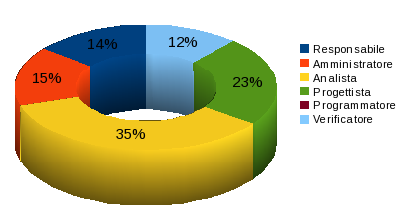
\includegraphics[width=300pt]{RR_RPP_Ore}

\begin{center}\textbf{Costo/Ruolo}
\end{center}
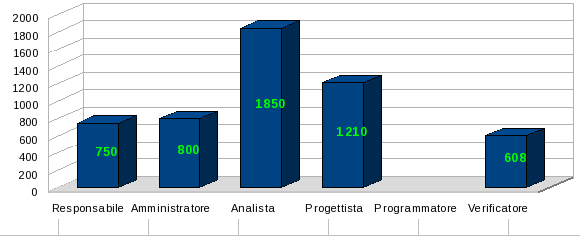
\includegraphics[width=350pt]{RR_RPP_Costi}
\newpage

\subsezione{Pianificazione economico-temporale RPP-RQ}
All'interno di questa fase avverranno le due iterazioni previste. I requisiti non funzionali verranno soddisfatti in modo trasversale rispetto alle due iterazioni. La prima iterazione inizier\`a immediatamente dopo l'RPP e si concluder\`a a met\`a della fase RPP-RQ. Al termine dell'iterazione verranno soddisfatti i requisiti funzionali obbligatori riguardanti il disegno di forme geometriche e testo e il relativo salvataggio/caricamento su file. Durante la seconda iterazione verranno soddisfatti i requisiti funzionali obbligatori non realizzati nella fase precedente. Potranno inoltre essere soddisfatti, in tutto o in parte, i requisiti funzionali desiderabili.
\\
\\
Preventivo relativo alla fase Revisione del progetto preliminare-Revisione di qualifica.
\begin{table}[h]
	\begin{center}
		  \begin{tabular}{|c|c|c|c|}
		 \hline 
		 \textbf{Ruolo} & \textbf{Ore di lavoro} & \textbf{Costo in euro}\\
		 \hline
		Responsabile & 33 & 990 \\
		Amministratore & 37 & 740\\
		Analista & 24 & 600\\
		Progettista & 89 & 1958\\
		Programmatore & 94 & 1504 \\
		Verificatore & 105 & 1680\\
        \hline
        \textbf{Totale} & \textbf{382} & \textbf{7472}\\
		\hline
		\end{tabular}
	\caption{Preventivo RPP-RQ} 
	\label{tab:tabella_RPP-RQ}
	\end{center}	
\end{table}

\newpage
\begin{center}\textbf{Ore/Ruolo}
\end{center}
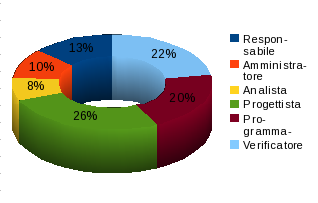
\includegraphics[width=300pt]{RPP_RQ_Ore}

\begin{center}\textbf{Costo/Ruolo}
\end{center}
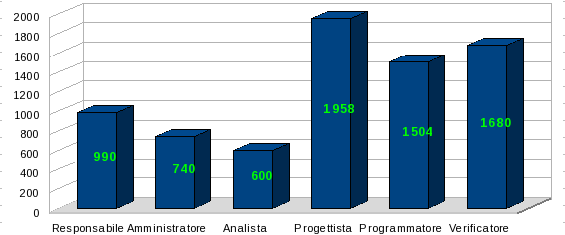
\includegraphics[width=350pt]{RPP_RQ_Costi}

\newpage

\subsezione{Pianificazione economico-temporale RQ-RA}
Preventivo relativo alla fase Revisione di qualifica-Revisione di accettazione.
\begin{table}[h]
	\begin{center}
		  \begin{tabular}{|c|c|c|c|}
		 \hline 
		 \textbf{Ruolo} & \textbf{Ore di lavoro} & \textbf{Costo in euro}\\
		 \hline
		Responsabile & 8 & 240 \\
		Amministratore & 10 & 200\\
		Analista & 0 & 0\\
		Progettista & 8 & 176\\
		Programmatore & 13 & 208 \\
		Verificatore & 16 & 256\\
        \hline
        \textbf{Totale} & \textbf{55} & \textbf{1080}\\
		\hline
		\end{tabular}
	\caption{Preventivo RQ-RA} 
	\label{tab:tabella_RQ-RA}
	\end{center}	
\end{table}



\begin{center}\textbf{Ore/Ruolo}
\end{center}
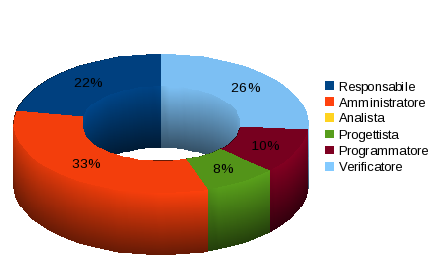
\includegraphics[width=300pt]{RQ_RA_Ore}

\begin{center}\textbf{Costo/Ruolo}
\end{center}
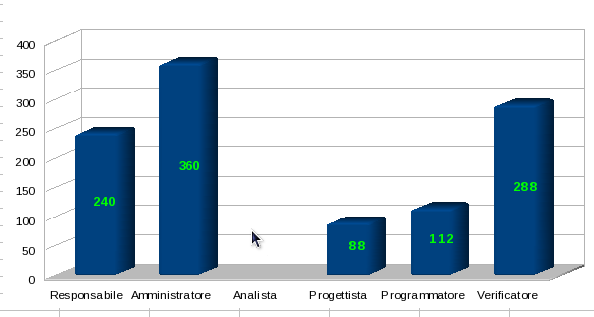
\includegraphics[width=350pt]{RQ_RA_Costi}

\subsezione{Distribuzione dei ruoli}
La distribuzione dei ruoli all'interno dell'azienda \`e stata realizzata in modo da permettere a tutti i membri di WebShape di ricoprire tutti i ruoli richiesti dal progetto, distribuendoli nel modo pi\`u equo possibile, rispettando i vincoli previsti dalle Assunzioni Iniziali. La distribuzione dei ruoli \`e meglio descritta nelle tabelle (\ref{tab:TabellaRotazRuoliUno}) e (\ref{tab:TabellaRotazRuoliDue}) a pagina ~\pageref{tab:TabellaRotazRuoliUno} ; \`e anche descritto il carico di lavoro/persona in ore nella tabella (\ref{tab:TabellaPrevPersOre}) a pagina ~\pageref{tab:TabellaPrevPersOre}.\\
La distribuzione del lavoro \`e visibile anche nei file Pianfica.png e PianificaRisorse.png consegnati assieme a questo documento.

Per conoscenza del cliente, \`e fornita anche una stima approssimativa dell'impiego orario rispetto ad ogni ruolo nella fase antecedente la RR. La retribuzione di tali ore non \`e a carico del committente, ma WebShape desidera mostrare quanto impegno sia stato investito nel progetto. La maggior parte degli sforzi \`e stata indirizzata nel dotare WebShape di metodi di lavoro adatti allo svolgimento del progetto, e per padroneggiare meglio con tali tecnologie.\\

\begin{table}[h]
	\begin{center}
		  \begin{tabular}{|c|c|c|c|}
		 \hline 
		 \textbf{Ruolo} & \textbf{Ore di lavoro} \\
		 \hline
		Responsabile & 20 \\
		Amministratore & 28 \\
		Analista & 32 \\
		Progettista & 10 \\
		Programmatore & 0 \\
		Verificatore & 12 \\
        \hline
        \textbf{Totale} & \textbf{102} \\
		\hline
		\end{tabular}
	\caption{Ore PRE-RR} 
	\label{tab:tabella_PRE_RR}
	\end{center}	
\end{table}

\newpage

\subsubsezione{Distribuzione per fase di progetto}
%%%%%%%%%%%%%%%%%%%%%%%%%%%%%%%%PRIMA PARTE TABELLA%%%%%%%%%%%%%%%%%%%%%%%%%%%%%%%%%%%%%%%%%%%%%
\begin{table}[!h]
	\begin{center}
		  \begin{tabular}
			  {|c|c|c|c|}
		 \hline
%%%%%%%%%%%%%%INTESTAZIONE COLONNE%%%%%%%%%%%%%%%%%%%%%%%%%%%%%%%%%%%%%%%%%%%%%%%%%%%%%%%%%%%%%%
			\multicolumn{3}{|c|}{ \textbf{Preventivo rotazione ruoli per fase di progetto} } \\
			\hline
			\textbf{Componente} & \multicolumn{2}{|c|}{ \textbf{FASE} } \\
			\hline
			& \textbf{RR-RPP} & \textbf{RPP-RQ} \\
			\hline
%%%%%%%%%%%%%%FINE INTESTAZIONE COLONNE%%%%%%%%%%%%%%%%%%%%%%%%%%%%%%%%%%%%%%%%%%%%%%%%%%%%%%%%%%%%%%
								     %  RR -RPP % RPP-RQ %  
			Bizzotto Piero & Resp.-Amm.-Progett.  & Analis.-Program.-Verif. \\
			\hline
			Carollo Mirko & Resp.-Amm.-Progett.  & Analis.-Program.-Verif.   \\
			\hline
			Cunico Marco & Analis.  & Resp.-Amm.-Progett.-Program.  \\
			\hline
			Dal Bosco Davide & Analis.  & Resp.-Amm.-Progett.-Program.-Verif.  \\
			\hline
			Dissegna Stefano & Analis.  & Resp.-Amm.-Progett.-Program.  \\
			\hline
			Geremia Mirco & Resp.-Amm.-Analis.-Verif.  & Progett.-Program.  \\
			\hline
			Rizzo Maurizio & Analis.-Progett.-Verif. & Resp.-Amm.-Program. \\
			\hline

%%%%%%%%%%% FINE PARTE DA MODIFICARE %%%%%%%%%%%%%%%%%%%%%%%%%%%%%%%%%%%%%%%%%%%%%%%%%%%%%%%%%%%
		\end{tabular}
	\caption{Preventivo rotazione ruoli per fase di progetto - prima parte} %INSERIRE DIDASCALIA - SE NECESSARIA - 
	\label{tab:TabellaRotazRuoliUno}
	\end{center}	
\end{table}
%%%%%%%%%%%%%%%%%%%%%%%%%%%%SECONDA PARTE TABELLLA%%%%%%%%%%%%%%%%%%%%%%%%%%%%%%%%%%%%%%%%%%%%%%
\begin{table}[!h]
	\begin{center}
		  \begin{tabular}
			  {|c|c|c|c|}
		 %\hline
%%%%%%%%%%%%%%INTESTAZIONE COLONNE%%%%%%%%%%%%%%%%%%%%%%%%%%%%%%%%%%%%%%%%%%%%%%%%%%%%%%%%%%%%%%
			%%\multicolumn{2}{|c|}{ \textbf{Preventivo rotazione ruoli per fase di progetto} } \\
			\hline
			\textbf{Componente} & \multicolumn{1}{|c|}{ \textbf{FASE} } \\
			\hline
			& \textbf{RQ-RA} \\
			\hline
%%%%%%%%%%%%%%FINE INTESTAZIONE COLONNE%%%%%%%%%%%%%%%%%%%%%%%%%%%%%%%%%%%%%%%%%%%%%%%%%%%%%%%%%%%%%%
								     % RQ-RA % 
			Bizzotto Piero & Resp.-Amm.   \\
			\hline
			Carollo Mirko & Verif.   \\
			\hline
			Cunico Marco & Amm. - Program.   \\
			\hline
			Dal Bosco Davide & Amm. - Program.  \\
			\hline
			Dissegna Stefano & Resp. - Progett.   \\
			\hline
			Geremia Mirco & Proget.   \\
			\hline
            Rizzo Maurizio  & Verif. \\
			\hline

%%%%%%%%%%% FINE PARTE DA MODIFICARE %%%%%%%%%%%%%%%%%%%%%%%%%%%%%%%%%%%%%%%%%%%%%%%%%%%%%%%%%%%
		\end{tabular}
	\caption{Preventivo rotazione ruoli per fase di progetto - seconda parte} %INSERIRE DIDASCALIA - SE NECESSARIA - 
	\label{tab:TabellaRotazRuoliDue}
	\end{center}	
\end{table}
\newpage
\subsubsezione{Distribuzione dei carichi di lavoro}
%Distribuzione del carico di lavoro per membro del gruppo.\\

\begin{table}[!h]
	\begin{center}
		  \begin{tabular}
			  {|c|c|c|c|c|c|c|c|}
		 \hline
%%%%%%%%%%%%%%INTESTAZIONE COLONNE%%%%%%%%%%%%%%%%%%%%%%%%%%%%%%%%%%%%%%%%%%%%%%%%%%%%%%%%%%%%%%
%			\multicolumn{3}{|c|}{ \multirow{2}{*}{ FASE RR - RPP } } \\
			\multicolumn{8}{|c|}{ \textbf{Preventivo carico persona ore} } \\
			\hline
			\textbf{Componente} & \multicolumn{7}{|c|}{ \textbf{RUOLO} } \\
			\hline
			& \textbf{Resp.} & \textbf{Amm.} & \textbf{Analis.} & \textbf{Progett.} & \textbf{Program.} & \textbf{Verif.}  & \textbf{Totale}\\
			\hline
%%%%%%%%%%%%%%FINE INTESTAZIONE COLONNE%%%%%%%%%%%%%%%%%%%%%%%%%%%%%%%%%%%%%%%%%%%%
								     %  RESP    % AMMIN  %  ANALISTA  %  PROGET. %  PROGRAM %    VERIF.   % TOTALE
			Bizzotto Piero       &  10   &  13  &  10   &   23  &  12   &  28   &  96\\ % R4
			\hline
			Carollo Mirko        &  10   &  13  &  10   &   22  &  12   &  29  &  96\\ % R5
			\hline
			Cunico Marco         &  10   &  19  &  21   &   20  &  18   &  7  &   95\\ % R2
			\hline
			Dal Bosco Davide     &  10   &  14  &  10   &   21  &  11   &  29  &  95\\ % R1
			\hline
			Dissegna Stefano     &  10   &  15  &  20   &   24  &  18   &  9  &  96\\ % R6
			\hline
			Geremia Mirco        &  11   &  10  &  17   &   14  &  13   &  30  &  95\\ % R7
			\hline		
			Rizzo Maurizio       &  10   &  14  &  10   &   20  &  12   &  29  &  95\\
			\hline
%%%%%%%%%%% FINE PARTE DA MODIFICARE %%%%%%%%%%%%%%%%%%%%%%%%%%%%%%%%%%%
		\end{tabular}
	\caption{Preventivo carico persona in ore} %INSERIRE DIDASCALIA - SE NECESSARIA - 
	\label{tab:TabellaPrevPersOre}
	\end{center}	
\end{table}

\newpage

\sezione{Consuntivi}
\subsezione{Fase RR-RPP}
\begin{table}[h]
	\begin{center}
		  \begin{tabular}{|c|c|c|c|}
		 \hline 
		 \textbf{Ruolo} & \textbf{Ore di lavoro} & \textbf{Costo in euro}\\
		 \hline
		Responsabile & 18 & 520 \\
		Amministratore & 44 & 880\\
		Analista & 86 & 2125\\
		Progettista & 39 & 858\\
		Programmatore & 0 & 0 \\
		Verificatore & 28 & 448\\
        \hline
        \textbf{Totale} & \textbf{215} & \textbf{4831}\\
		\hline
		\end{tabular}
	\caption{Consuntivo RR-RPP} 
	\label{tab:cons_RR-RPP}
	\end{center}	
\end{table}

\begin{center}\textbf{Ore/Ruolo}
\end{center}
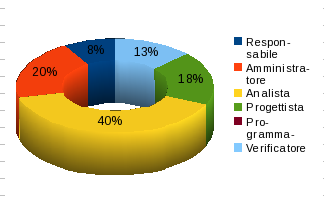
\includegraphics[width=300pt]{Cons-RR-RPP2}
\newpage

\begin{center}\textbf{Costo/Ruolo}
\end{center}
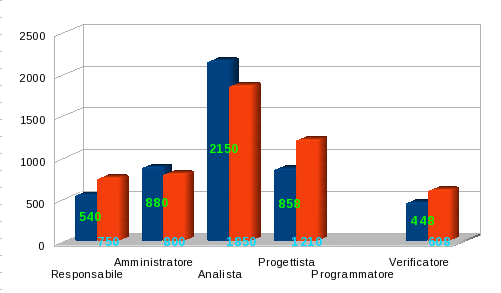
\includegraphics[width=350pt]{Cons-RR-RPP1}


\begin{table}[!h]
	\begin{center}
		  \begin{tabular}
			  {|c|c|c|c|c|c|c|c|}
		 \hline
%%%%%%%%%%%%%%INTESTAZIONE COLONNE%%%%%%%%%%%%%%%%%%%%%%%%%%%%%%%%%%%%%%%%%%%%%%%%%%%%%%%%%%%%%%
%			\multicolumn{3}{|c|}{ \multirow{2}{*}{ FASE RR - RPP } } \\
			\multicolumn{8}{|c|}{ \textbf{Consuntivo Ore/Ruolo} } \\
			\hline
			\textbf{Componente} & \multicolumn{7}{|c|}{ \textbf{RUOLO} } \\
			\hline
			& \textbf{Resp.} & \textbf{Amm.} & \textbf{Analis.} & \textbf{Progett.} & \textbf{Program.} & \textbf{Verif.}  & \textbf{Totale}\\
			\hline
%%%%%%%%%%%%%%FINE INTESTAZIONE COLONNE%%%%%%%%%%%%%%%%%%%%%%%%%%%%%%%%%%%%%%%%%%%%
								     %  RESP    % AMMIN  %  ANALISTA  %  PROGET. %  PROGRAM %    VERIF.   % TOTALE
			Bizzotto Piero &  6   &  13 &  0   &   28  &  0   &  0  &  47 \\ % R4
			\hline
			Carollo Mirko &  8   &  24  &  0  &  11   &  0   &  0   &  43\\ % R5
			\hline
			Cunico Marco    &  0   &  0  &  29   &  0   &  0  &  0   &  29\\ % R2
			\hline
			Dal Bosco Davide   &  0   &  0   &  12   &  0   &   0  &  0  &  12\\ % R1
			\hline
			Dissegna Stefano        &  0  &  0   & 27  &  0   &  0  &  0  &  27\\ % R6
			\hline
			Geremia Mirco   &   2  &  6   &  13  &  0  &  0   &  26   &  47\\ % R7
			\hline	
			Rizzo Maurizio  &  0  &  0  &  20  &  10  &  0  &  15  &  45 \\ %R3
			\hline	
%%%%%%%%%%% FINE PARTE DA MODIFICARE %%%%%%%%%%%%%%%%%%%%%%%%%%%%%%%%%%%
		\end{tabular}
	\caption{Consuntivo carico/persona RR-RPP} %INSERIRE DIDASCALIA - SE NECESSARIA - 
	\label{tab: ConsPersOre_RR-RPP}
	\end{center}	
\end{table}

Come si pu\`o vedere dai dati precendentemente elencati si sono rivelate necessarie alcune modifiche rispetto al preventivo presentato:
sono stati richiesti sforzi maggiori dal ruolo di amministratore per l'attuazione di piani e procedure di gestione della qualit\`a ed
analista per analizzare pi\`u a fondo i requisiti. I ruoli di responsabile, progettista e verificatore hanno invece richiesto minori
risorse del previsto anche grazie al buon lavoro svolto nella fase PRE-RR.

\newpage

\subsezione{Fase RPP-RQ}
\begin{table}[h]
	\begin{center}
		  \begin{tabular}{|c|c|c|c|}
		 \hline 
		 \textbf{Ruolo} & \textbf{Ore di lavoro} & \textbf{Costo in euro}\\
		 \hline
		Responsabile & 31 & 930 \\
		Amministratore & 42 & 840\\
		Analista & 12 & 300\\
		Progettista & 82 & 1804\\
		Programmatore & 103 & 1648 \\
		Verificatore & 97 & 1552\\
        \hline
        \textbf{Totale} & \textbf{367} & \textbf{7074}\\
		\hline
		\end{tabular}
	\caption{Consuntivo RPP-RQ} 
	\label{tab:cons_RPP-RQ}
	\end{center}	
\end{table}

\begin{center}\textbf{Ore/Ruolo}
\end{center}
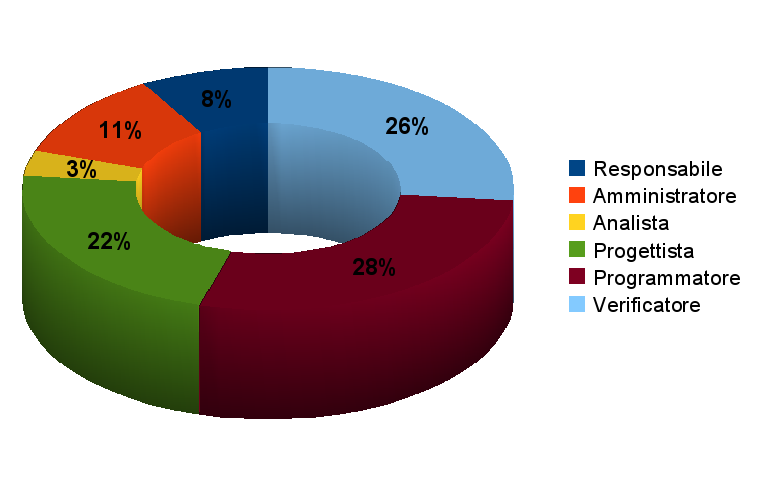
\includegraphics[width=300pt]{Cons-RPP-RQ1}
\newpage

\begin{center}\textbf{Costo/Ruolo}
\end{center}
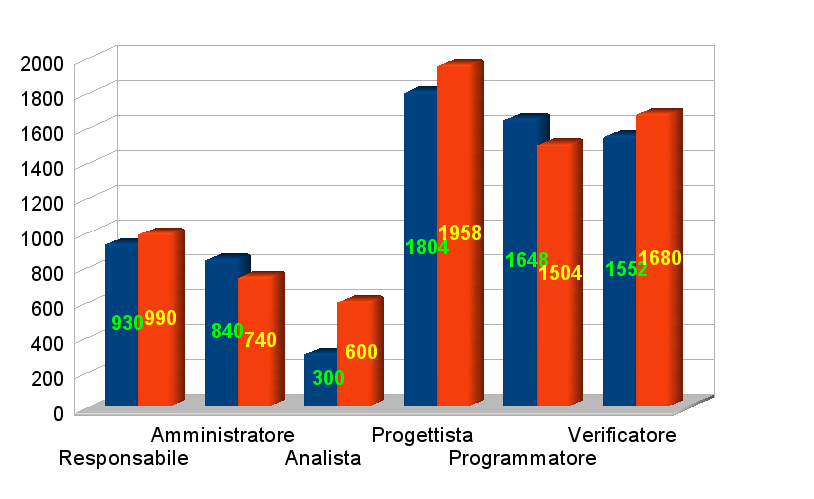
\includegraphics[width=350pt]{Cons-RPP-RQ2}


\begin{table}[!h]
	\begin{center}
		  \begin{tabular}
			  {|c|c|c|c|c|c|c|c|}
		 \hline
%%%%%%%%%%%%%%INTESTAZIONE COLONNE%%%%%%%%%%%%%%%%%%%%%%%%%%%%%%%%%%%%%%%%%%%%%%%%%%%%%%%%%%%%%%
%			\multicolumn{3}{|c|}{ \multirow{2}{*}{ FASE RPP - RQ} } \\
			\multicolumn{8}{|c|}{ \textbf{Consuntivo Ore/Ruolo} } \\
			\hline
			\textbf{Componente} & \multicolumn{7}{|c|}{ \textbf{RUOLO} } \\
			\hline
			& \textbf{Resp.} & \textbf{Amm.} & \textbf{Analis.} & \textbf{Progett.} & \textbf{Program.} & \textbf{Verif.}  & \textbf{Totale}\\
			\hline
%%%%%%%%%%%%%%FINE INTESTAZIONE COLONNE%%%%%%%%%%%%%%%%%%%%%%%%%%%%%%%%%%%%%%%%%%%%
							%RESP    % AMMIN  %  ANALISTA  %  PROGET. %  PROGRAM %    VERIF.   % TOTALE
			Bizzotto Piero 		&  0  &  0  &  4  &  0  &  13 &  28 &  45 \\ % R4
			\hline
			Carollo Mirko 		&  0  &  0  &  12 &  0  &  10 &  31 &  49\\ % R5
			\hline
			Cunico Marco    	&  7  &  11 &  0  &  23 &  16 &  0  &  57\\ % R2
			\hline
			Dal Bosco Davide   	&  8  &  5  &  0  &  16 &  11 &  38 &  78\\ % R1
			\hline
			Dissegna Stefano    &  8  &  10 &  0  &  20 &  23 &  0  &  61\\ % R6
			\hline
			Geremia Mirco   	&  0  &  0  &  0  &  23 &  18 &  0  &  41\\ % R7
			\hline	
			Rizzo Maurizio  	&  8  &  16 &  0  &  0  &  12 &  0  &  36\\ %R3
			\hline	
%%%%%%%%%%% FINE PARTE DA MODIFICARE %%%%%%%%%%%%%%%%%%%%%%%%%%%%%%%%%%%
		\end{tabular}
	\caption{Consuntivo carico/persona RPP-RQ} %INSERIRE DIDASCALIA - SE NECESSARIA - 
	\label{tab: ConsPersOre_RPP-RQ}
	\end{center}	
\end{table}

Si pu\`o notare dai dati che in generale \`e stato richiesto un impegno leggermente minore rispetto a quanto previsto, in particolare il ruolo di Analista ha richiesto meno impegno, poich\`e nel preventivo l'azienda si era tutelata su questo campo inserendo ore extra per eventuali problemi. Sono state utilizzate meno ore anche per quel che riguarda la verifica, dove hanno giocato un ruolo importante gli stumenti adottati e le modalit\`a di automazione della gestione degli errori, che hanno permesso di velocizzare i processi di verifica. L'unico ruolo che ha richiesto un maggiore impegno \`e stato quello del Programmatore, poich\`e si sono riscontrati problemi non previsti nell'implementazione di alcuni elementi.

\subsubsezione{Implicazioni del consuntivo}
In questa fase il progetto \`e in fase di completamento e ci si aspetta un lavoro nella fase seguente per quel che riguarda la codifica e la relativa verifica. Il preventivo relativo alla fase RQ-RA \`e stato quindi aggiornato per questo motivo, e soprattutto per l'acquisizione e l'integrazione di un nuovo membro all'interno dell'azienda.


\sezione{Gestione del Piano di Progetto}
\subsezione{Obiettivi}
L'obiettivo del documento denominato "Piano di Progetto" \`e distribuire le risorse durante l'arco temporale 
contenente lo sviluppo del capitolato d'appalto. Questa distribuzione ovviamente deve rispettare i vincoli presentati 
nella sezione "Assunzioni Iniziali".

\sezione{Analisi e Gestione dei Rischi}
In questa sezione saranno presi in considerazione i possibili problemi che potrebbero sorgere durante la realizzazione del progetto, sia dal punto di vista della pianificazione delle fasi di lavoro, che da quello di eventuali rischi relativi alla tecnologia usata. Per ogni rischio \`e presente (\textit{in italico}) la situazione attuale.\\
I punti di rischio da noi identificati e valutati sono i seguenti:
\begin{itemize}
\item \textbf{Rischi inerenti al modello di ciclo di vita incrementale}\\
\`E molto importante effettuare una corretta scelta delle attivit\`a, da coordinare durante le varie fasi di lavoro. \textit{La pianificazione delle attivit\`a ha permesso di seguire questo modello di ciclo di vita, e l'azienda \`e riuscita a svolgere il progetto con le iterazioni previste.}
\item \textbf{Pianificazione e distribuzione dei ruoli}\\
Un punto fondamentale al quale bisogna prestare molta attenzione \`e la suddivisione dei ruoli e la sua gestione. Ogni componente dovr\`a assumere tutti i ruoli durante le varie fasi di progetto. Questo pu\`o portare ad una scarsa specializzazione dei membri dell'azienda, ma si tratta di un vincolo didattico indispensabile. \textit{Ogni componente ha ricoperto quasi tutti i ruoli; ai membri che non hanno svolto alcuni ruoli questi gli saranno assegnati come previsto nella fase seguente, in modo da riuscire a soddisfare il vincolo didattico richiesto.}
\item \textbf{Mancanza del personale}\\
Essendo l'azienda composta da sei membri, nell'eventualit\`a che uno di questi non possa pi\`u partecipare alle attivit\`a di progetto, c'\`e comunque la possibilit\'a che l'azienda abbia un numero sufficiente di persone per continuare il lavoro sotto le ipotesi e le stime preventivate. In tutti gli altri casi possibili, l'azienda WebShape porter\`a comunque a termine il suo lavoro. \textit{Il suddetto rischio non \`e pi\`u presente in seguito all'integrazione di un nuovo componente. L'azienda \`e ora composta da sette membri.}
\item \textbf{Compatibilit\`a e portabilit\`a del prodotto}\\
Il prodotto finale, come da Requisiti, dovr\`a risultare funzionante sui pi\`u moderni {\underline{browser}} in circolazione. Questo fatto \`e per\`o  a discrezione dell'utente finale, il quale deve essere consapevole della non retrocompatibilit\`a del prodotto, e quindi anche la portabilit\`a risulta essere  a sua discrezione.
\item \textbf{Funzionalit\`a del prodotto}\\
Essendo il prodotto finale utilizzato da un qualsiasi tipo di utente finale, \`e necessario prestare attenzione a come il prodotto si presenta, rendendo l'accessibilit\`a a tutte le sue funzioni semplice e immediata. \textit{Il prodotto presenta un'interfaccia grafica intuitiva, dotata di toolbar laterale e men\`u a tendina per facilitare l'interazione con l'utente.}
\end{itemize}			

\end{document}
